\subsection{Приливы и отливы}
Ускорение в центре Земли($T$) считется по слейдующей формуле: \begin{equation}\omega_T=\frac{GM}{r^2}
\end{equation}
Где $m$ --- масса Луны, $r^2$ --- расстояние между центрами Земли и Луны. Ускорения в точках A и B равны:
\begin{equation}\omega_A=\frac{GM}{(r-R)^2} \text{ и } \omega^B=\frac{GM}{(r+R)^2}
\end{equation}
Где $R$ --- радиус Земли. Ускорение точки A относительно точки T равно:
\begin{equation}\omega_A-\omega_T=Gm\frac{2rR-R^2}{(r-R)^2r^2}
\end{equation}
Так как $R\ll r$, то \begin{equation}\omega_A-\omega_T=\frac{Gm2R}{r^3}
\end{equation}

Под действием лунного притяжения водная оболочка Земли принимает форму эллипсоида, который вытянут по направлению к Луне. Близ точек $А$ и $В$ будет прилив, а у точек $F$ и $D$ --- отлив (Рис.7).
\begin{center}
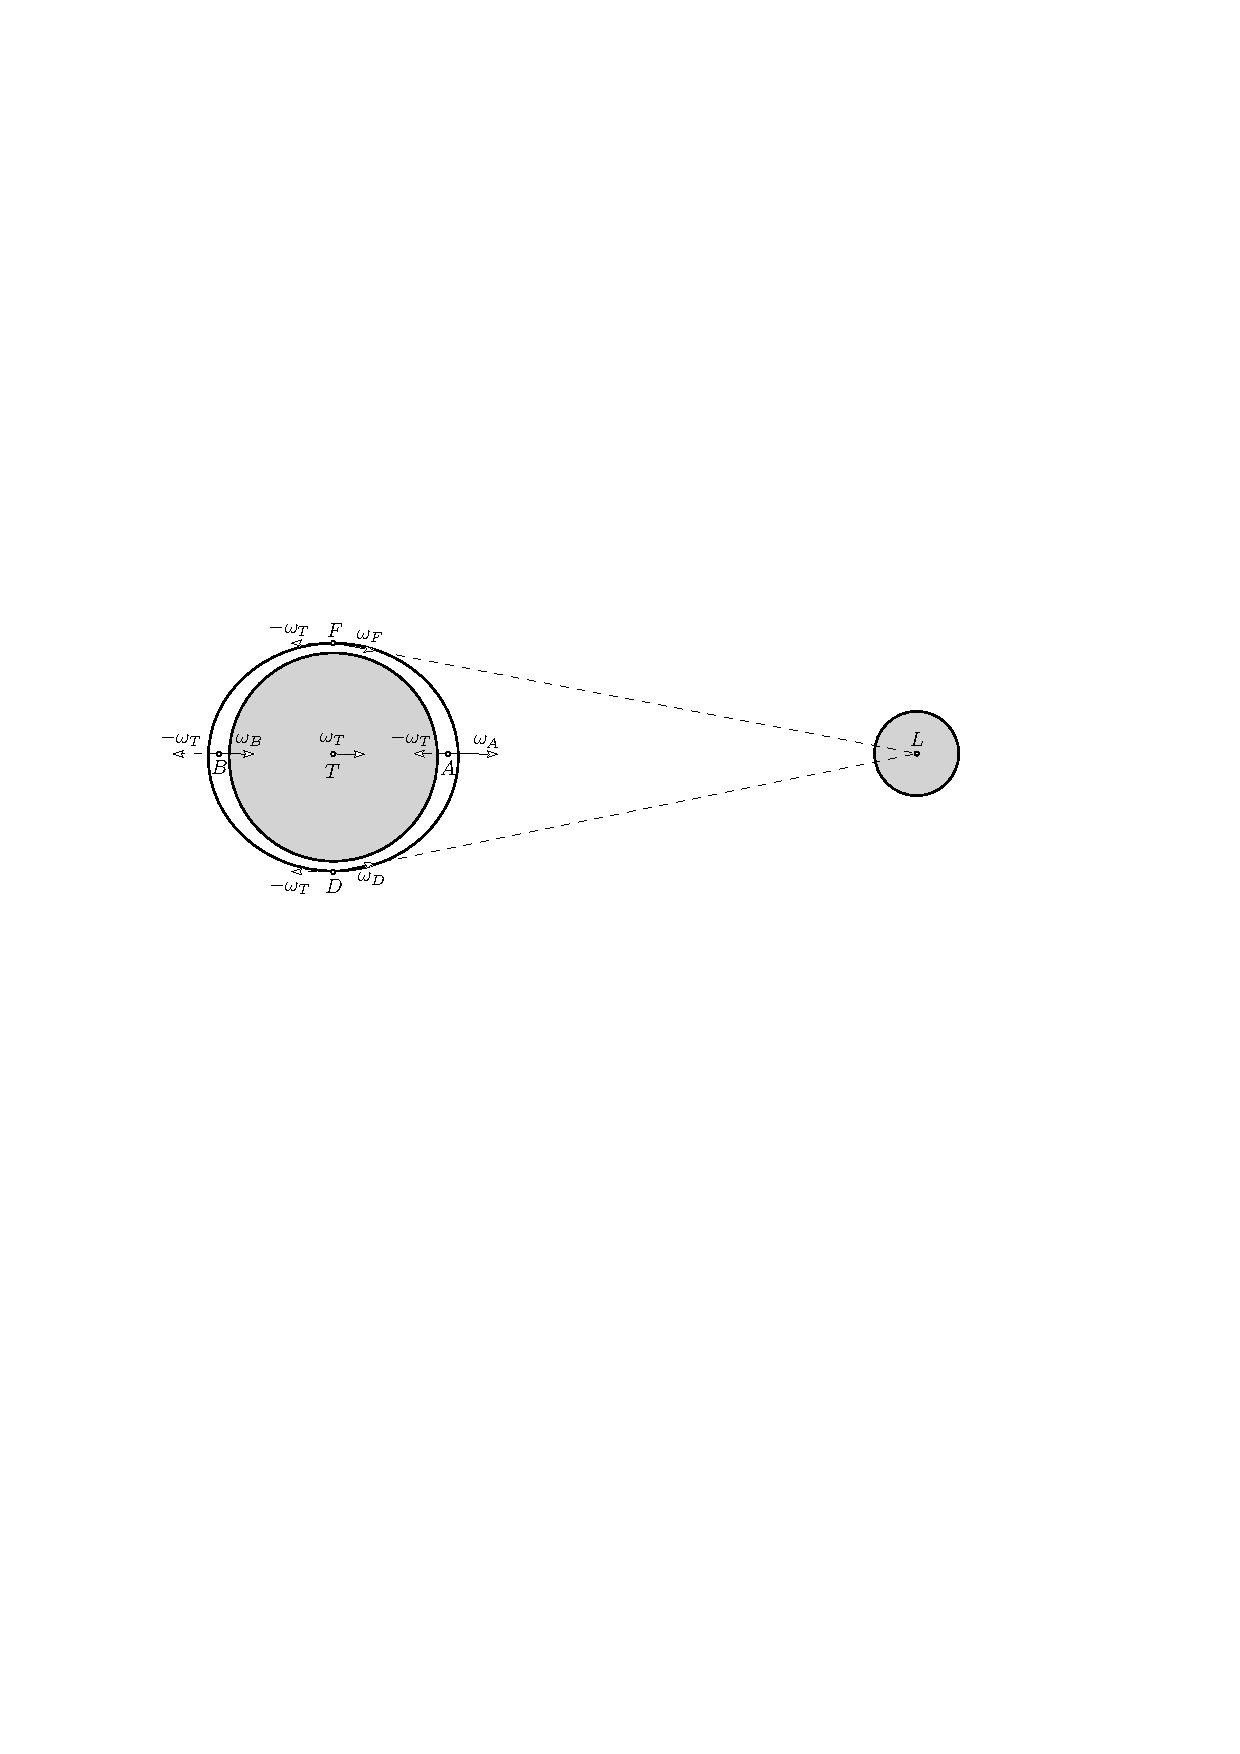
\includegraphics[width = 1\textwidth]{Ebb_flow}
\begin{figure}[h!]
\caption{К объяснению приливных сил}
\end{figure}
\end{center}
